\documentclass[]{report}

\title{To explore the mechanism that allows music recognition apps to work. }
\author{Cephas Yeung}
\date{10/2/2025}

% MIT License

% Copyright (c) [2024] [Cephas Yeung]

% Permission is hereby granted, free of charge, to any person obtaining a copy
% of this software and associated documentation files (the "Software"), to deal
% in the Software without restriction, including without limitation the rights
% to use, copy, modify, merge, publish, distribute, sublicense, and/or sell
% copies of the Software, and to permit persons to whom the Software is
% furnished to do so, subject to the following conditions:

% The above copyright notice and this permission notice shall be included in all
% copies or substantial portions of the Software.

% THE SOFTWARE IS PROVIDED "AS IS", WITHOUT WARRANTY OF ANY KIND, EXPRESS OR
% IMPLIED, INCLUDING BUT NOT LIMITED TO THE WARRANTIES OF MERCHANTABILITY,
% FITNESS FOR A PARTICULAR PURPOSE AND NONINFRINGEMENT. IN NO EVENT SHALL THE
% AUTHORS OR COPYRIGHT HOLDERS BE LIABLE FOR ANY CLAIM, DAMAGES OR OTHER
% LIABILITY, WHETHER IN AN ACTION OF CONTRACT, TORT OR OTHERWISE, ARISING FROM,
% OUT OF OR IN CONNECTION WITH THE SOFTWARE OR THE USE OR OTHER DEALINGS IN THE
% SOFTWARE.
% 
% GitHub link:
% https://github.com/seabass6969/latex-template
\usepackage[utf8]{inputenc}

\usepackage{amsmath, amsfonts, amsthm, graphicx, geometry, lipsum, subfigure}
\usepackage{blindtext}
\makeatletter
\let\runauthor\@author
\let\runtitle\@title
\makeatother

\usepackage{pdfpages}
\usepackage{appendix}

\usepackage[nottoc, numbib]{tocbibind}
% \usepackage[comma]{natbib}
\usepackage[
  backend=biber,
  style=numeric, % default
  % style=alphabetic,
  % style=authoryear,
]{biblatex}

\usepackage{verbatim, fancyvrb}
\usepackage{fancyhdr, lastpage}
\pagestyle{fancy}
\lhead{\runtitle}
\rhead{\runauthor}
\usepackage{listings}


% \patchcmd{\chapter}{\thispagestyle{plain}}{\thispagestyle{fancy}}{}{}
% \expandafter\patchcmd\csname chapter*\endcsname{\thispagestyle{plain}}{\thispagestyle{fancy}}{}{}
\usepackage[Sonny]{fncychap}
\usepackage{xcolor-material}
\usepackage[svgnames]{xcolor}
\usepackage{tikz, tcolorbox}
\tcbuselibrary{listings,breakable}
\usepackage{longtable}
\usepackage{hyperref}

\hypersetup {
    colorlinks=true,
    linkcolor=blue,
    urlcolor=red,
    citecolor=RoyalBlue
}
\renewcommand\theHtable{Appendix.\thetable}

\newcommand{\trademark}{\textsuperscript{\textregistered}}
\newcommand\TBox[3][]{%
  \tikz\node[draw,ultra thick,text width=#2,align=left,#1] {#3};}


% \usepackage{harvard}
\patchcmd{\thebibliography}{\chapter*}{\section}{}{}

\usetikzlibrary{matrix}
\definecolor{15}{HTML}{000000}
\definecolor{14}{HTML}{111111}
\definecolor{13}{HTML}{222222}
\definecolor{12}{HTML}{333333}
\definecolor{11}{HTML}{444444}
\definecolor{10}{HTML}{555555}
\definecolor{9}{HTML}{666666}
\definecolor{8}{HTML}{777777}
\definecolor{7}{HTML}{888888}
\definecolor{6}{HTML}{999999}
\definecolor{5}{HTML}{AAAAAA}
\definecolor{4}{HTML}{BBBBBB}
\definecolor{3}{HTML}{CCCCCC}
\definecolor{2}{HTML}{DDDDDD}
\definecolor{1}{HTML}{EEEEEE}
\definecolor{0}{HTML}{FFFFFF}

\tikzset{ 
table/.style={
  matrix of nodes,
  row sep=-\pgflinewidth,
  column sep=-\pgflinewidth,
  nodes={rectangle,draw=black,fill=0,minimum size=1cm,align=center},
  nodes in empty cells
  }
}
\tikzset{
    block/.style ={ rectangle, 
draw, fill=white,  text centered, minimum size=1cm, nodes in empty cells,
  row sep=-\pgflinewidth,
  column sep=-\pgflinewidth,
fill=green}
    }

\usetikzlibrary{shapes.misc}


\addbibresource{Shazam/Shazam.bib}
\begin{document}

\begin{titlepage}
   \centering
   {\Large \bfseries {\runtitle} \bigbreak}
   {\scriptsize \small{\runauthor} \bigbreak}
   \includegraphics[scale=0.3]{screenshots/main_screen.png}\par\vspace{1cm}
\end{titlepage}
% \maketitle
\tableofcontents
\newpage
\chapter*{Abstract}
\textit{For the purpose of this project, the replica of a music recognition app is created.}

\textit{The algorithm first creates an almost unique fingerprint for each audio file from the spectrogram. Which the fingerprints are added to a database as a hashed value.}

\textit{When record songs through the interface, the algorithm repeats the process of fingerprinting, but instead compare hash value with matched songs.}
\chapter{Introduction}

In the modern world, billions and billions of songs are created, and you might want to recognize song that you don't know. This article answer how does modern music recognition app work.

My aim for this research is to understand and replicate how modern day music recognition algorithms work. 

From using a very concrete source of a patent created by the original founder and Chief Scientist of Shazam\trademark (Now part of Apple Inc\trademark.)\cite{newnham_interview_2023}.

This source allows a great understanding of the background information of the program. 

During the creation process, it was created using different resources to make the resource (e.g: patent, research paper) and also methods to test the success criteria set out by the algorithm. 

In conclusion, the program is successful.
\chapter{Methodology / Design Choice}
The artefact is separated in different pieces. (Structure: \autoref{fig:overall_arch}).

The software is run inside a container as the patent suggested that although not limited to any particular system, it is preferred for it to be run in a “Distributed system”. But by containerize the program, it allows it to happen.

Next, the program is separated into two parts. The web app part allows user to interact graphically. (Screenshots: \autoref{fig:screenshot:main}). And most importantly the main algorithm.

The program first records the audio, this is done through the web app.  


And the main algorithm collects the audio file and sent to an algorithm to "fingerprint" the piece of music. The algorithm consist of spectrogram produced from the SciPy signal library \cite{virtanen_scipy_2020} where it uses STFT (Short-time Fourier Transform is a variation of the Fast Fourier transform built for making spectrogram). In this case, Fast Fourier transform are used to convert from time and amplitudes domain to a representation in the frequency domain. It's illustrated in \autoref{fig:fft}. \cite{noauthor_fast_2025} And the data are processed using the library of NumPy\cite{harris_array_2020}. 


An array of data from the spectrogram are being filtered through maximum filter in the SciPy library \cite{virtanen_scipy_2020}. The two arrays are compared to use to pick peak points. The peaks are used to construct the pairs. Which is illustrated in \autoref{fig:listfiltering} and \autoref{fig:pairspicking}.

The pairs of points hashed using the default hashing function (Hashing function is a set of things to do to make an output that is always the same length from some other input data. Hash functions and their associated hash tables are used in data storage to access data in a fast time. \cite{noauthor_hash_2024}) from python which generate an almost unique hash values in the program. \autoref{fig:hash}


The hash point is than placed into a database alongside with its song name and where the point A's real time. The song data (metadata) such as author and copyright detail are placed in a different database.

When the user record the sample through the user interface created, the recording sample is sent to the server. It is processed where it applies the same algorithm from above. First it constructs a spectrogram, create and compare it with a filtered spectrogram, peak point are picked and hash values are created, the hash value searched inside the `points` table. 

The list of successfully matched song are than going through the process of "scoring". The score calculated by constructing a histogram with the point A's real time value. The score is assigned to each song with the highest value in each histogram. This is because the peak point of some songs are the same for a completely different song. And this includes background noise where the algorithm could mistake it to be a different song.

\cite{wang_systems_2013,macleod_abracadabra_nodate,yang_music_2001}
\chapter{Testing method}
The program is tested using the method described in this paper \cite{yang_music_2001} and also a meeting from  \hyperref[meeting:2]{professional}. An evidence from all the song from (most) of the fingerprinted music collection is used to test the program, this is so that it reduce the likelihood of a flawed test. Classical music is used because there is lower chance for creating copyright issues.

The test have increasing level of difficulty:
\label{chapter:test_methods:methods}
\begin{itemize}
    \item Test 1: original song file (unmodified digital file)
    \item Test 2: original song file but shifted 
    \item Test 3: original song file but with controlled level of noise. (E.g.: a sine wave)
    \item Test 4: original song file but played over the air and recorded.
    \item Test 5: original song but perform by different people.
    \item Test 6: transposed song \label{t:test_transposed}
\end{itemize}
The test results is inside \autoref{fig:table_of_testing_result}.
The program overall worked as expected but test 6 doesn't work because this algorithm is not designed for this.

\chapter{Discussion}

As discussed in \hyperref[t:test_transposed]{the test conducted}, this artefact is not capable to detect a transposed song. Because this song only matches the exact frequency that the song produces. 

One way that the problem can solve is to change the mechanism entirely to not rely purely on the raw frequency data, instead by using the MIDI file of the song which contains a series of message like note. \cite{amandaghassaei_what_nodate} Then from it, create a database of melody. Which can recognise songs from it by recording the song and passing into the algorithm to process for results. This allows a wider error range for recognizing song such as made from "humming". \cite{ghias_query_1995, yang_music_2001}. However, this would make the algorithm costly and slow to run.

In addition, extra research might be needed to improve the speed, making it more commercially viable which is the goal set out by the Shazam\trademark team. \cite{wang_systems_2013}

The research can also be further extended not limited to searching for songs, such as searching for patten inside picture or video.

\chapter{Conclusion}

Further research might be needed into improving the accuracy, making it able to recognise variation of the same song. \cite{yang_music_2001}

In conclusion, It met the expectation of the project end goal which are tested using a vigorous testing method set out by a professional opinion and an article. 


\printbibliography[heading=bibintoc, title={Bibliography}]
\addtocontents{toc}{\vspace{1em}\hrule\vspace{1em}}

\appendix
% \bibliographystyle{plain}
\chapter{Figures}
\begin{figure}[h!]
\label{fig:overall_arch}
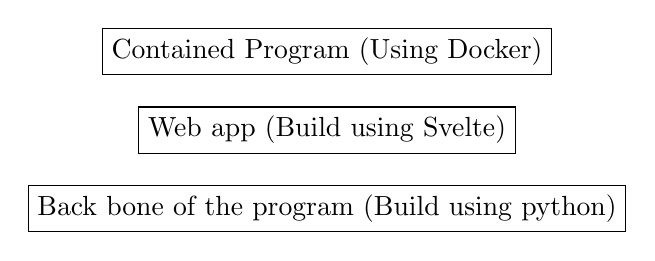
\begin{tikzpicture}
\node[draw] at (0,0) {Contained Program (Using Docker)};
\node[draw] at (0,-1) {Web app (Build using Svelte)};
\node[draw] at (0, -2) {Back bone of the program (Build using python)};
\end{tikzpicture}
\end{figure}
\begin{figure}
    \centering
    \includegraphics[scale=0.2]{figures/FourierTransform.png}
    \includegraphics[scale=0.2]{figures/FourierTransformed.png}
    \caption{Fast Fourier Transform as an example through transforming the top signal in to representation in the frequency domain at the bottom.}
    \label{fig:fft}
\end{figure}

% automatically generated by the script in the /music_recognition_main/figure_generation/arraydiagram.py
\begin{figure}
    \centering
    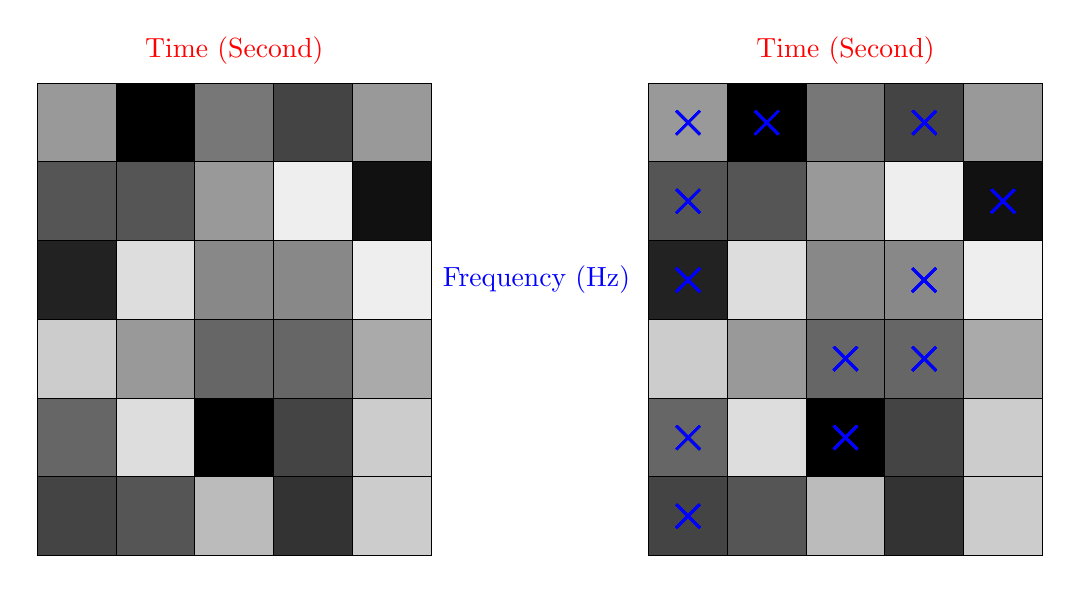
\begin{tikzpicture}
    \matrix (m) [table]
    {
 |[fill=6]| & |[fill=15]| & |[fill=8]| & |[fill=11]| & |[fill=6]| \\
 |[fill=10]| & |[fill=10]| & |[fill=6]| & |[fill=1]| & |[fill=14]| \\
 |[fill=13]| & |[fill=2]| & |[fill=7]| & |[fill=7]| & |[fill=1]| \\
 |[fill=3]| & |[fill=6]| & |[fill=9]| & |[fill=9]| & |[fill=5]| \\
 |[fill=9]| & |[fill=2]| & |[fill=15]| & |[fill=11]| & |[fill=3]| \\
 |[fill=11]| & |[fill=10]| & |[fill=4]| & |[fill=12]| & |[fill=3]| \\
    };
    \matrix (mat) [table, right=2.5cm of m]
    {
 |[fill=6]| & |[fill=15]| & |[fill=8]| & |[fill=11]| & |[fill=6]| \\
 |[fill=10]| & |[fill=10]| & |[fill=6]| & |[fill=1]| & |[fill=14]| \\
 |[fill=13]| & |[fill=2]| & |[fill=7]| & |[fill=7]| & |[fill=1]| \\
 |[fill=3]| & |[fill=6]| & |[fill=9]| & |[fill=9]| & |[fill=5]| \\
 |[fill=9]| & |[fill=2]| & |[fill=15]| & |[fill=11]| & |[fill=3]| \\
 |[fill=11]| & |[fill=10]| & |[fill=4]| & |[fill=12]| & |[fill=3]| \\
    };
        \node [above=3pt of m-1-3] (test) {\textcolor{Red}{Time (Second)}};
        \node [above=3pt of mat-1-3] (test) {\textcolor{Red}{Time (Second)}};
        \node [left=3pt of mat-3-1] (test) {\textcolor{Blue}{Frequency (Hz)}};

        \draw [blue,thick] plot[only marks,mark=x,mark size=6pt] (mat-1-1); 
        \draw [blue,thick] plot[only marks,mark=x,mark size=6pt] (mat-1-2); 
        \draw [blue,thick] plot[only marks,mark=x,mark size=6pt] (mat-1-4); 
        \draw [blue,thick] plot[only marks,mark=x,mark size=6pt] (mat-2-1); 
        \draw [blue,thick] plot[only marks,mark=x,mark size=6pt] (mat-2-5); 
        \draw [blue,thick] plot[only marks,mark=x,mark size=6pt] (mat-3-1); 
        \draw [blue,thick] plot[only marks,mark=x,mark size=6pt] (mat-3-4); 
        \draw [blue,thick] plot[only marks,mark=x,mark size=6pt] (mat-4-3); 
        \draw [blue,thick] plot[only marks,mark=x,mark size=6pt] (mat-4-4); 
        \draw [blue,thick] plot[only marks,mark=x,mark size=6pt] (mat-5-1); 
        \draw [blue,thick] plot[only marks,mark=x,mark size=6pt] (mat-5-3); 
        \draw [blue,thick] plot[only marks,mark=x,mark size=6pt] (mat-6-1); 
    \end{tikzpicture}
    \caption{Illustrating the picking of points, the darker the box, the darker the amplitude (value) represents}
    \label{fig:listfiltering}
\end{figure}


\begin{figure}
    \centering
    \includegraphics[scale=0.2]{figures/Delta_distance_demo.png}
    \caption{}
    \label{fig:pairspicking}
\end{figure}

\begin{figure}
    \centering
    \small
        \begin{tabular}{|c|c|c|c|c|}
            \hline
            Point A (Hz) & Point B (Hz) & Time delta (s) & Point A time (s) & Track UUID \\
            \hline
            20.1 & 302.1 & 1.8 & 0.3 & $ea47a3c5$\\
            \hline
            \multicolumn{3}{|c|}{$2388532207457024332$} & 2.1 & $ea47a3c5$\\
            \hline
        \end{tabular}
    \caption{Demonstrate / example of how item are hashed. \cite{macleod_abracadabra_nodate}}
    \label{fig:hash}
\end{figure}

\chapter{Testing results}
\begin{figure}
Test 1: (tested on 100\% of the song library)

\begin{tabular}{|c|c|c|}
\hline
filepath & passed & SUBTOTAL \\
\hline
test/test\_1.py & 46 & 46 \\
\hline
TOTAL & 46 & 46 \\
\hline
\end{tabular}

Test 2: (tested on 100\% of the song library)

\begin{tabular}{|c|c|c|}
\hline
filepath & passed & SUBTOTAL \\
\hline
test/test\_2.py & 46 & 46 \\
\hline
TOTAL & 46 & 46 \\
\hline
\end{tabular}

Test 3: (tested on 100\% of the song library)

\begin{tabular}{|c|c|c|c|}
\hline
filepath & passed & failed & SUBTOTAL \\
\hline
test/test\_3.py & 34 & 12 & 46 \\
\hline
TOTAL & 34 & 12 & 46 \\
\hline
\end{tabular}

Test 4:
Most works (Only tested 40\% of the song library)

Test 5:
Most failed (Only tested 20\% of the song library)

Test 6:
All failed (Only tested 10\% of the song library)
    \centering
    \caption{test result table}
    \label{fig:table_of_testing_result}
\end{figure}

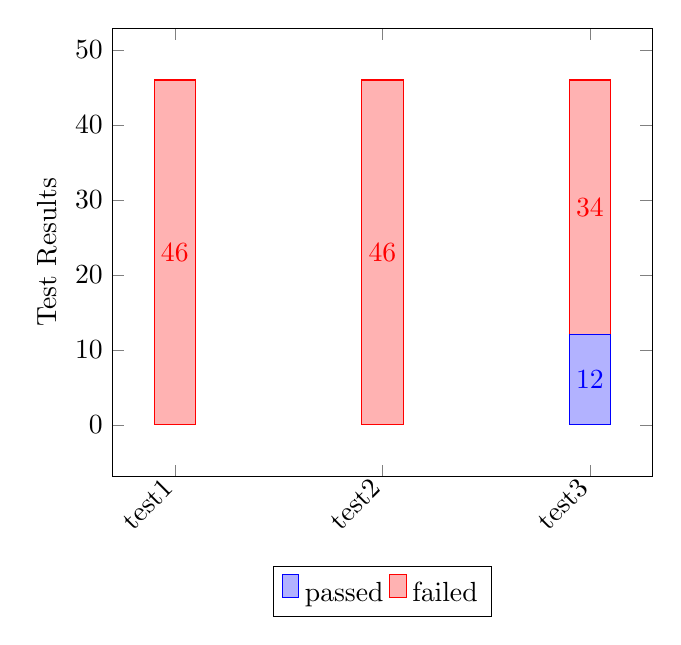
\begin{tikzpicture}
\begin{axis}[
    ybar stacked,
	bar width=15pt,
	nodes near coords,
    enlargelimits=0.15,
    legend style={at={(0.5,-0.20)},
      anchor=north,legend columns=-1},
    ylabel={Test Results},
    symbolic x coords={test1, test2, test3},
    xtick=data,
    x tick label style={rotate=45,anchor=east},
    ]
    \addplot+[ybar] plot coordinates {(test1,0) (test2,0) (test3, 12)};
    \addplot+[ybar] plot coordinates {(test1,46) (test2,46) (test3, 34)};
\legend{\strut passed, \strut failed}
\end{axis}
\end{tikzpicture}

\chapter{Screenshots}
\begin{figure}[htbp!]
\centering
\subfigure[]{\includegraphics[scale=0.18]{screenshots/main_screen.png}\label{screenshot:main:home}}
\subfigure[]{\includegraphics[scale=0.18]{screenshots/main_screen_idle_perm.png}\label{screenshot:main:perm}}
\subfigure[]{\includegraphics[scale=0.18]{screenshots/main_screen_idle_denied_permission.png}\label{screenshot:main:error}}
\label{fig:screenshot:main}
\caption{(a) "Home", (b)(c) "Microphone permission are disabled"}
\end{figure}

\begin{figure}[htbp!]
\centering
\subfigure[]{\includegraphics[scale=0.18]{screenshots/unrecognizable_tooshort.png}\label{screenshot:recognize:too_short}}
\subfigure[]{\includegraphics[scale=0.18]{screenshots/unrecognizable_song.png}\label{screenshot:recognize:no_song}}
\subfigure[]{\includegraphics[scale=0.18]{screenshots/recognizable_song.png}\label{screenshot:main:working}}
\label{fig:screenshot:recognize}
    \caption{(a) "Too Short", (b) "No song", (c) "Recognized song (e.g: Prelude by Bach)"}
\end{figure}
All the figures are simulated to the size of an iPhone\trademark SE display.

\chapter{Meeting logs}
\section*{Meeting with the supervisor at \date{25 November 2024}}
Summary: 

Improve on the part A of the production logs, with more details on the titles described and what resources I will be using (such as the URLs should be provided), the timescale and what is involve. 

As things I should be including to create a great project is the benefit that this might bring to the society and the impact.  

And a plan to see what I should be sending or showing to the examiner in the future such as:  

\begin{itemize}
    \item Send product log 
    \item Presentation of the artefact 
    \item Evidence of the artefact 
    \item Critical bibliography 
    \item Place that in the Appendix and write a reference back to the appendix through the production log.  
\end{itemize}
\section*{Meeting with a professional at \date{13 January 2025}}
Summary:

I explained the background details during the meeting.

I have explained that the program can only detect sounds from following test that I conducted such as:
\begin{itemize}
    \item A test where there are no modifications to the original sound,
    \item A test where the song has cropped and reduced to a smaller size.
    \item A test where there is a constant noise generated by a program with a constant sine wave in the background.
    \item A test where the songs are mixed with a normal acceptable background noise such as coughing.
\end{itemize}

All of those above works as expected.

However the test that I did by recording when the sound is played on a music player on a different device doesn’t work.

As an additional note, he has mentioned that the program is slow because of a reason which might be caused by the hash point not being an integer, as the hash value using integer is faster than using string as hash. (It was diagnosed with a slow database reading speed prior to the meeting).

The project has concluded as partially successful from the results produced from the searching algorithm. 

\textbf{Summary of Improvement I need to make from the project.}

I should use a different hashing algorithm for the fingerprinting part of the program.

Round up the frequency, and the changes in time that are fed into the hashing algorithm.

\textbf{Additional note:}

The meetings are conducted with the consent of the professional. (With regards to the ethical issues)

The professional is my computer science teacher, as he has a decent qualification of a university degree.
\chapter{Critical Bibliography}
\begin{longtable}{|p{4.5cm}|c|p{5cm}|p{2.5cm}|}
    \hline 
    Sources & & Critics & Notes \\
    \hline
    \fullcite{amandaghassaei_what_nodate} & \cite{amandaghassaei_what_nodate} & 
    This tutorial article is indented to provide a really basic definition about the MIDI file. 
    & \\
    \hline
    \fullcite{noauthor_fast_2025} & \cite{noauthor_fast_2025} &
    This Wikipedia is indented to provide a really basic definition about the fast Fourier Transform. As Wikipedia might not be the most credible source. And it might have inaccuracy. So this source is not used extensively.
    & \\
    \hline 
    \fullcite{ffmpeg_developers_ffmpeg_nodate} & \cite{ffmpeg_developers_ffmpeg_nodate} &
    This program is indented to be used in the program. This program extensively used in audio processing inside the code as an assistant / helper tool. This tool is also extensively used for other audio related processing. 
    & Utilized only in the code\\
    \hline 
    \fullcite{ghias_query_1995} & \cite{ghias_query_1995} &
    This conference article provide a discussion point on how to make the artefact if I want to do it differently. This source is credible to an extent as it's written by ACM which is a scientific and educational computing society. However, it might be slightly outdated (published date 1995) as there might be more information about this.
    & \\
    \hline 
    \fullcite{harris_array_2020} & \cite{harris_array_2020} &
    This program is indented to be used in the program. This program extensively used in data analysis. It's an industry standard tool to analysis array in all fields, such as research.
    & Utilized only in the code\\
    \hline 
    \fullcite{noauthor_hash_2024} & \cite{noauthor_hash_2024} &
    This Wikipedia is indented to use to provide a really basic definition about the hash function. As Wikipedia might not be the most credible source. And it might have inaccuracy. So this source is not used extensively.
    & \\
    \hline 
    \fullcite{macleod_abracadabra_nodate} & \cite{macleod_abracadabra_nodate} &
    This blog post is important because this includes much more details that the original article from the Shazam company. However, this does not mean this blog post are accurate as this is from written from a perspective of the original creator. But the writer is partially qualified to write about this topic as the writer work as a software engineer at Bloomberg and a graduate of University of Edinburgh.
    & \\
    \hline 
    \fullcite{newnham_interview_2023} & \cite{newnham_interview_2023} &
    This interview give an insight into the creator of Shazam Avery Wang's identity, which his source is used as concrete source in the program. \cite{wang_systems_2013, wang_industrial-strength_2003}
    & \\
    \hline 
    \fullcite{virtanen_scipy_2020} & \cite{virtanen_scipy_2020} &
    This program is indented to be used in the program. This program extensively used in solving mathematical problem and scientific tool. And it's an industry standard programming interface for solving mathematical problem and analysing scientific problem.
    & Utilized only in the code\\
    \hline 
    \fullcite{wang_industrial-strength_2003} & \cite{wang_industrial-strength_2003} &
This is the original article explaining from a prospective of the creator. This article creates a basic understanding of how the basics works. They have a detail analysis of recognition rate and the performance associated. However, the article is missing from explaining the method of how they create Spectrogram, and the algorithm they are using to create it. There might be changes to the modern day algorithm that the product is using, this might be due to the age of this paper being published in 2003. And since now the company are acquired by Apple Inc.
    & \\
    \hline 
    \fullcite{wang_systems_2013} & \cite{wang_systems_2013} &
    This source is very credible and concrete, as the original program Shazam are based on it. It is created by the founder and principle scientist of Shazam. Inside the source there are also figures attached to it. This patent is cited (as of February 2025) 771 times. It's being used in various different field, most notability social media companies and big tech companies such as Google, Snap. However, the source might not be as relevant because the patent are outdated and expired.
    & \\
    \hline 
    \fullcite{yang_music_2001} & \cite{yang_music_2001} &
    This source provides resources mainly how to test the artefact. This report are also written by the Stanford University which is a very credible source and provides great information.
    & \\
    \hline 
\end{longtable}

\chapter{Timetable}
See the landscape table file after this page.
\begin{itemize}
    \item \textcolor{Green}{Green done means on time}
    \item \textcolor{Orange}{Orange done means not on time}
\end{itemize}
I choose to use timetable target set by week because it allows for more streamline approach to time management.
\includepdf[pages=-, landscape=true]{timetable_exported.pdf}

\end{document}
